Simulacemi zjistěte tyto parametry tranzistorů NMOS a PMOS:

\begin{enumerate}
    \item {\bf Navrhněte proudovou referenci podle obr. 1a)} (bez startovacího obvodu). Předpokládané napětí na výstupu je \(1.2 V\) - toto napětí zde připojte v simulaci. Výstupní proud je \(50 \mu A\) 
    a proudy v jádru reference jsou \(10 \mu A\). Postupně:    
    \begin{enumerate}
        \item vypočítejte parametry všech součástek v obvodu (\textcolor{red}{P - výpočty ve formátu obecná rovnice, dosazení, výsledek}).
        \item proveďte analýzu {\bf.op} - zobrazte si proudy ve větvích a napětí ve všech uzlech  (\textcolor{red}{P - schéma se zvýrazněnými U/I dle předlohy})
        \item a zobrazte si Spice Output log a zkontrolujte parametry polovodičových součástek (\textcolor{red}{P - printscreen pracovních bodů tranzistorů ze Spice Output Log})
    \end{enumerate}
    \begin{figure}[h]
        \centering
        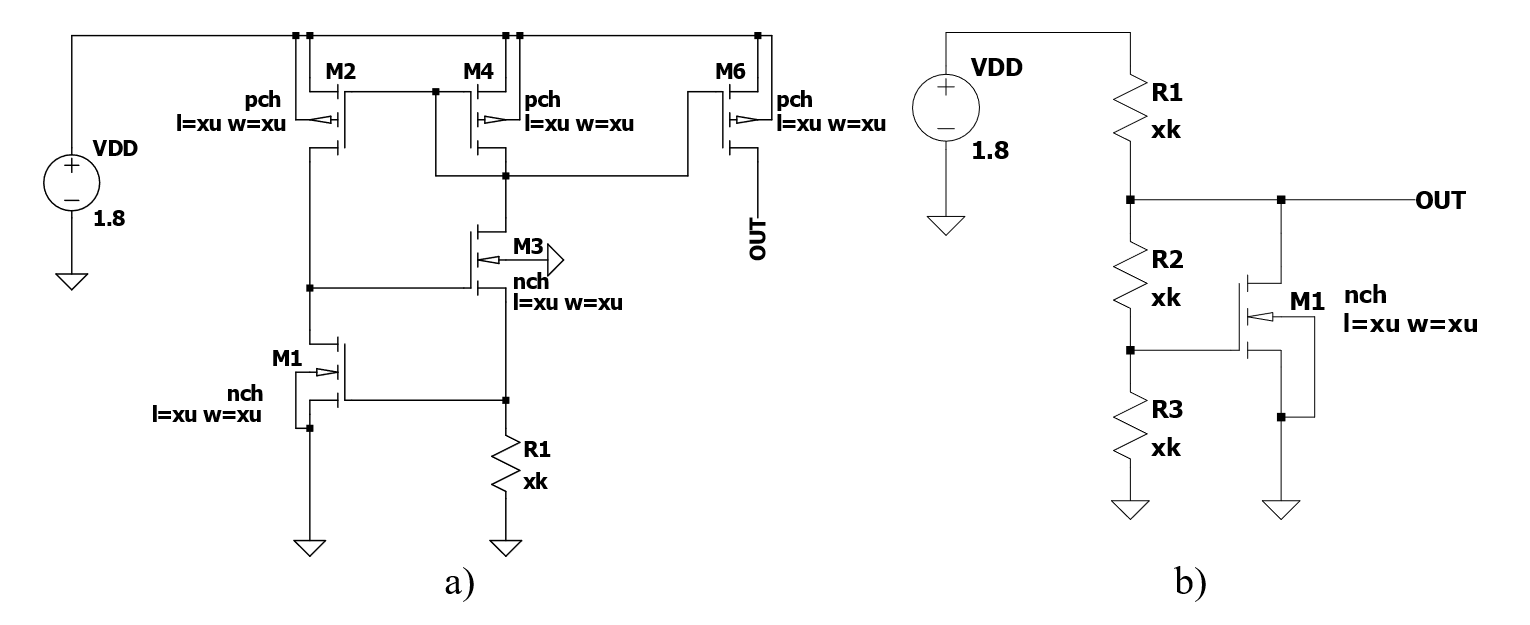
\includegraphics[height=0.3\textheight]{text/img/zadani.png}
        \caption{\label{fig:sch_zadani} Proudový zdroj s kaskádovým PZ}
    \end{figure}
    \item {\bf Navrhněte napěťovou reference podle obr. 1b.} Požadované výstupní napětí je \(1.2 V\), proudová spotřeba obvodu pak \(50 \mu A\)
    \begin{itemize}
        \item vypočítejte parametry všech součástek v obvodu  (\textcolor{red}{P - výpočty ve formátu obecná rovnice, dosazení, výsledek}).
        \item proveďte analýzu {\bf.op} - zobrazte si proudy ve větvích a napětí ve všech uzlech  (\textcolor{red}{P - schéma se zvýrazněnými U/I dle předlohy})
        \item a zobrazte si Spice Output log a zkontrolujte parametry tranzistoru NMOS (\textcolor{red}{P - printscreen ze Spice Output Log})
    \end{itemize}
    \item {\bf Pro napěťovou referenci z úlohy 2) použijte namísto odporu R1 proudovou referenci z úlohy 1)}
    \begin{enumerate}
        \item proveďte analýzu {\bf.op} - zobrazte si proudy ve větvích a napětí ve všech uzlech  (\textcolor{red}{P - schéma se zvýrazněnými U/I dle předlohy})
        \item krokujte napájecí napětí a sledujte výstupní referenční napětí. Odečtěte změnu tohoto napětí mezi \(UDD = 1.6 V\) a \(UDD = 2 V\) (\textcolor{red}{P - grafický výstup z LTspice s umístěnými kurzory a viditelnou tabulkou s jejich pozicí})  
    \end{enumerate}
\end{enumerate}
